\documentclass{article}

% Mise en page
\usepackage[scale=0.75]{geometry}
% Pied de page
\usepackage{fancyhdr}
\pagestyle{fancy}
\renewcommand{\headrulewidth}{0pt}
% Interligne après les paragraphes
\setlength{\parskip}{1.5ex}

% Langues
\usepackage[french]{babel}
\usepackage[utf8]{inputenc}
\usepackage[T1]{fontenc}
\usepackage{eurosym}

% Images
\usepackage{graphicx}
\usepackage{rotating}

% Code source
\usepackage{listings}
\usepackage{color}

\newcommand{\code}[1]{\lstinputlisting[title=#1.java]{../laFac.com/src/laFac/#1.java}}

\definecolor{dkgreen}{rgb}{0,0.6,0}
\definecolor{gray}{rgb}{0.5,0.5,0.5}
\definecolor{mauve}{rgb}{0.58,0,0.82}

\lstset{
  frame=tb,
  language=Java,
  aboveskip=3mm,
  belowskip=3mm,
  showstringspaces=false,
  columns=flexible,
  basicstyle={\small\ttfamily},
  numbers=left,
  stepnumber=5,
  numberstyle=\tiny\color{gray},
  keywordstyle=\color{blue},
  commentstyle=\color{dkgreen},
  stringstyle=\color{mauve},
  breaklines=true,
  breakatwhitespace=true
  tabsize=4,
  literate=
    {á}{{\'a}}1 {é}{{\'e}}1 {í}{{\'i}}1 {ó}{{\'o}}1 {ú}{{\'u}}1
    {Á}{{\'A}}1 {É}{{\'E}}1 {Í}{{\'I}}1 {Ó}{{\'O}}1 {Ú}{{\'U}}1
    {à}{{\`a}}1 {è}{{\'e}}1 {ì}{{\`i}}1 {ò}{{\`o}}1 {ò}{{\`u}}1
    {À}{{\`A}}1 {È}{{\'E}}1 {Ì}{{\`I}}1 {Ò}{{\`O}}1 {Ò}{{\`U}}1
    {ä}{{\"a}}1 {ë}{{\"e}}1 {ï}{{\"i}}1 {ö}{{\"o}}1 {ü}{{\"u}}1
    {Ä}{{\"A}}1 {Ë}{{\"E}}1 {Ï}{{\"I}}1 {Ö}{{\"O}}1 {Ü}{{\"U}}1
    {â}{{\^a}}1 {ê}{{\^e}}1 {î}{{\^i}}1 {ô}{{\^o}}1 {û}{{\^u}}1
    {Â}{{\^A}}1 {Ê}{{\^E}}1 {Î}{{\^I}}1 {Ô}{{\^O}}1 {Û}{{\^U}}1
    {œ}{{\oe}}1 {Œ}{{\OE}}1 {æ}{{\ae}}1 {Æ}{{\AE}}1 {ß}{{\ss}}1
    {ç}{{\c c}}1 {Ç}{{\c C}}1 {ø}{{\o}}1 {å}{{\r a}}1 {Å}{{\r A}}1
    {€}{{\euro{}}}1 {£}{{\pounds}}1
}


\begin{document}

\newcommand{\HRule}{\rule{\linewidth}{0.5mm}}

\begin{titlepage}
\begin{center}


\includegraphics[width=0.5\textwidth]{polytech}~\\[1cm]

\textsc{\LARGE Conception Objet}\\[1.5cm]

\textsc{\Large Projet de Programmation Orienté Objet}\\[0.5cm]

% Title
\HRule \\[0.4cm]
{ \huge \bfseries LaFac.com \\[0.4cm] }
\HRule \\[1.5cm]

% Author and supervisor
\begin{minipage}{0.4\textwidth}
\begin{flushleft} \large
\emph{Auteur:}\\
Jeremie \textsc{Bosom}\\
Erwan \textsc{Chaussy}\\
Léo \textsc{Dellouve}
\end{flushleft}
\end{minipage}
\begin{minipage}{0.4\textwidth}
\begin{flushright} \large
\emph{Professeur:} \\
M.~Frederic \textsc{Voisin}
\end{flushright}
\end{minipage}

\vfill

% Bottom of the page
{\large \today}

\end{center}
\end{titlepage}

\rhead{Conception Objet - LaFac.com}
\lfoot{
\includegraphics[scale=0.3]{polytech.jpg}}
\rfoot{BOSOM - CHAUSSY - DELLOUVE}

\section*{Introduction}

Afin de travailler la conception de systèmes réels, nous avons créé un modélisé un pseudo-site de vente en ligne.\par
L'implémentation s'est faite en Java et nous devions répondre à plusieurs contraintes, à savoir un système de gestion de personnes, de produits et de différentes offres applicables.

\clearpage

\section*{Diagramme de classe}

La classe principale de notre projet est la classe Contexte.
Il s'agit d'un \textbf{Singleton}, c'est-à-dire qu'il n'en existe qu'une seule instance dans le programme.
Ce contexte représente, en quelques sorte, la base de donnée que possèderait un site réel.
Si nous devions nous passer de celui-ci, nous basculerions les offres employés dans le statut \emph{Employe} qui deviendrait alors un \textbf{Singleton}.
Nous ajouterions aussi un autre \textbf{Singleton} qui contiendrait les \emph{OffreFidelites} pour les \emph{Adherents}.
\par
Parmi les autre \textbf{Design Pattern} utilisés nous avons le design \textbf{State} pour les statuts des \emph{Personnes}.
En effet, nous devions laisser la possibilité aux \emph{Personnes} de changer de \emph{Statut} en cours d'exécution, rendant ce design indispensable.
\par
Un autre \textbf{Design Pattern} que nous utilisons est celui de l'\textbf{Observer}.
Il consiste en une classe qui en ``observe'' une autre.
Ainsi, lors d'un changement de l'instance de cette classe, l'\textbf{Observer} associé effectuera une suite d'actions prédéfinies.
Dans notre projet, la classe \emph{Alerte} est un \textbf{Observer} sur la classe \emph{Panier}.
Lors d'un changement de celui-ci, l'\emph{Alerte} affichera un message.
\par
Enfin nous avons fait le choix d'une liaison faible entre les \emph{Produits} et les \emph{Offres} afin que la modification d'une offre n'impacte pas le produit en lui même.
En effet, une offre doit connaitre le produit sur lequel elle s'applique, mais le contraire n'est pas vrai.
De plus, cela évite qu'un changement dans les \emph{Offres} ne produise une erreurs ailleurs, améliorant la robustesse de notre programme.
\par
La généricité du langage Java est utilisée lors des affichages.
En effet, chaque type de \emph{Produit} à un affichage personnalisé, tout comme les \emph{Offres}, qui est géré lors de l'exécution du programme.
Celui-ci va chercher la bonne fonction à appeler et la définir dans la classe abstraite force la redéfinition de celle-ci dans les sous-classes.

{
Hook (le crochet) n'est pas un DP mais un idiome. Il consiste à définir une méthode template dans
la classe du haut et à laisser les sous-classes redéfinir les méthodes virtuelles qui les
concernent. C'est quand même une bonne habitude de programmation qui peut être citée ici,
par exemple pour implémenter l'affichage des offres en laissant chaque classe afficher les
spécificités (nombre de produits, ...) qui les concernent.
}

\begin{sidewaysfigure}[ht]
	\vfill\hfill % Centrage sur la page
	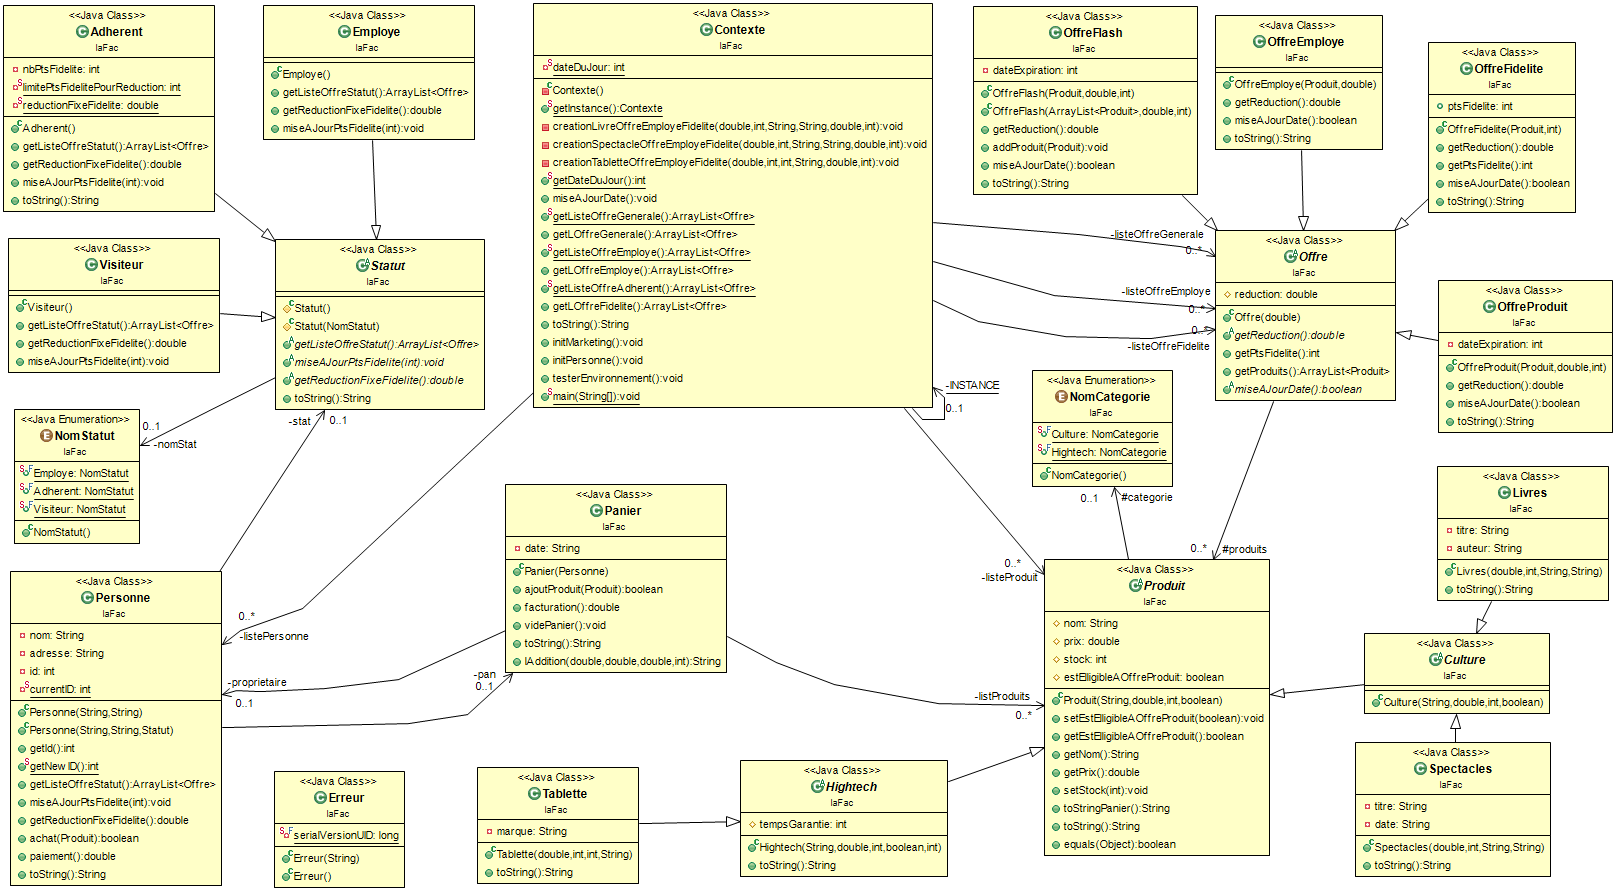
\includegraphics[scale=0.36]{diagUML.png}
	\hfill\vfill % Centrage sur la page
	\caption{Diagramme de classe}
\end{sidewaysfigure}

\clearpage % Force l'affichage des images flottantes avant de passer une page

\section*{Diagrammes de séquences}

Nous avons décidé de détailler les interactions entre les classes lors la création du contexte et lors de la facturation du panier.

\begin{figure}[ht]
	\begin{center}
		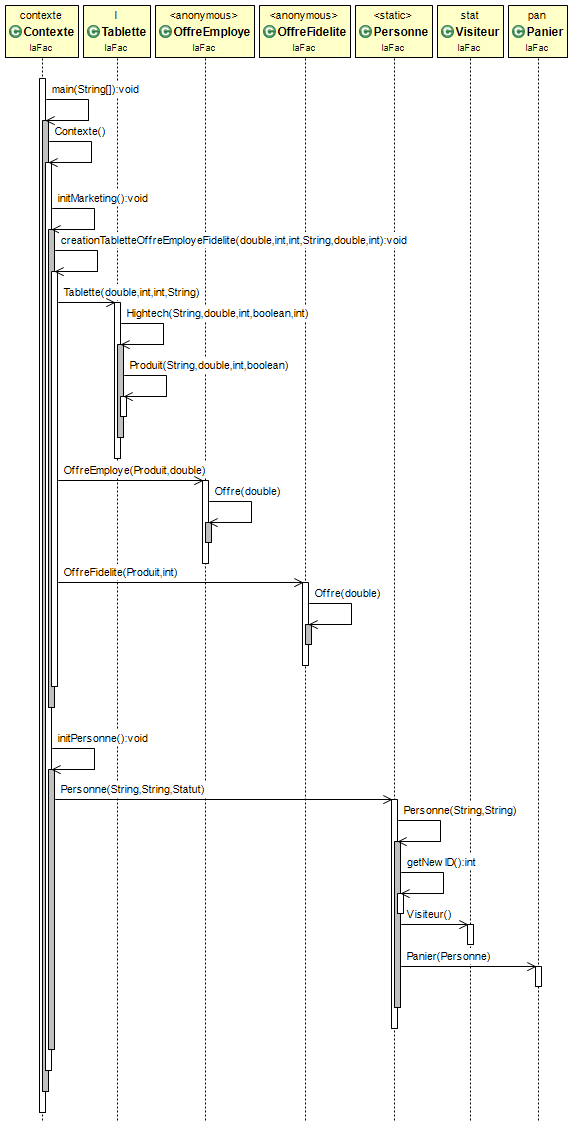
\includegraphics[scale=0.38]{creationContexte.png}
		\caption{Diagramme de séquence de la création du contexte}
	\end{center}
\end{figure}


\begin{figure}[ht]
	\begin{center}
		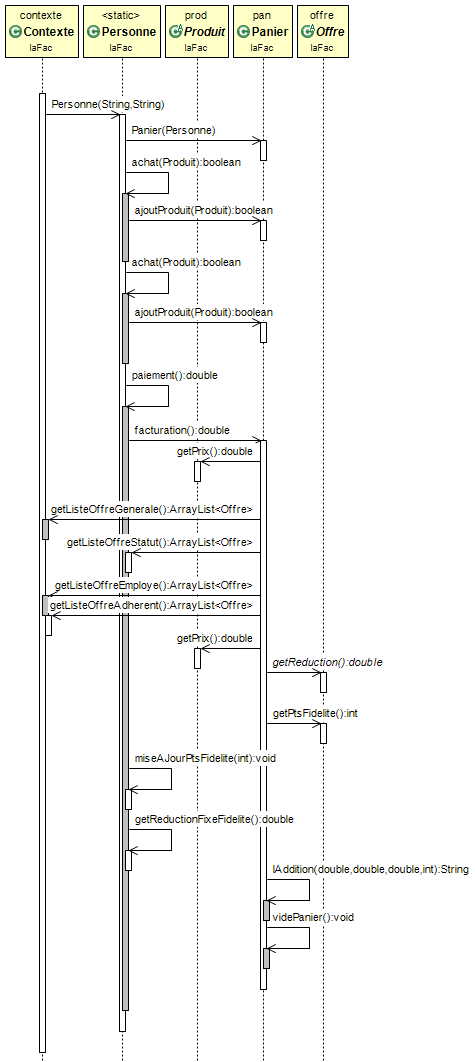
\includegraphics[scale=0.5]{ajouteProduitFactu.png}
		\caption{Diagramme de séquence de la facturation}
	\end{center}
\end{figure}


\clearpage % Force l'affichage des images flottantes avant de passer une page

\vfill
\section*{Conclusion}

Ce projet nous a permis de réfléchir à un problème concret, mettant en œuvre les connaissances acquises durant le cours.
\par
Nous avons utilisé plusieurs \textbf{Design Pattern}, afin de répondre aux différentes contraintes du sujet,
et la généricité du langage afin que les interactions entre les objets soient le plus simple et le plus clair possible, tout en offrant une possibilité d'évolution du code.
\par
En résumé, il s'agissait d'un exercice enrichissant qui nous aura permis d'acquérir de nouvelles connaissances.

 \clearpage
 
\section*{Annexe - Code source}

\subsection*{Contexte}
% Contexte
\code{Contexte}
\code{Alerte}
% Panier
\code{Panier}

\subsection*{Personnes}
% Personnes
\code{Personne}
\code{NomStatut}
\code{Statut}
\code{Adherent}
\code{Employe}
\code{Visiteur}

\subsection*{Produits}
% Produits
\code{Produit}
\code{NomCategorie}
\code{Culture}
\code{Hightech}
\code{Livres}
\code{Spectacles}
\code{Tablette}

\subsection*{Offres}
%Offres
\code{Offre}
\code{OffreEmploye}
\code{OffreFidelite}
\code{OffreFlash}
\code{OffreProduit}


\end{document}